%===============================================================================
% $Id: ifacconf.tex 19 2011-10-27 09:32:13Z jpuente $  
% Template for IFAC meeting papers
% Copyright (c) 2007-2008 International Federation of Automatic Control
%===============================================================================
\documentclass[a4paper]{ifacconf}

\usepackage{graphicx,amsmath,url}      % include this line if your document contains figures
\usepackage[round]{natbib}             % required for bibliography
\usepackage{algorithm}%
\usepackage{algorithmicx}%
\usepackage{algpseudocode}%
\usepackage{subcaption}
\usepackage{multirow}
\usepackage{booktabs}
%===============================================================================
% Choose the language of the manuscript.
% If in English, choose 
% \def\portugues{0} 
%
% If in Portuguese or Spanish, choose
\def\portugues{1} 
%
% If the above line is commented, it is assumed manuscript in English:
% ===============================================================
\ifx\portugues\undefined
\def\portugues{0}
\fi

\usepackage[T1]{fontenc}
\usepackage[utf8]{inputenc}
\usepackage{ae}

\if\portugues0
   \usepackage[english]{babel}
\else
   \usepackage[brazil]{babel}
\fi

\begin{document}

\if\portugues1
% =====================================================================
% =====================================================================
% USE THIS PART IF THE TEXT IS IN PORTUGUESE
% =====================================================================
% If the manuscript is in Spanish, please change the texts adequately.
% =====================================================================
% 
\selectlanguage{brazil}

\begin{frontmatter}

\title{Aprimoramento de Metaheurísticas para Otimização da Cadeia de Suprimentos de Pistache}

\author[First]{Raissa Gon\c{c}alves Diniz} 
\author[Second]{Andr\'e Costa Batista} 

\address[First]{Laboratório de Pesquisa Operacional e Sistemas Complexos, Universidade Federal de Minas Gerais, Brasil (e-mail: raissagd@ufmg.br).}
\address[Second]{Departamento de Engenharia Elétrica, Universidade Federal de Minas Gerais, Av. Ant\^onio Carlos 6627, Belo Horizonte, 31270-010, Minas Gerais, Brasil (e-mail: andre-costa@ufmg.br).}

\renewcommand{\abstractname}{{\bf Resumo:~}}   

\begin{abstract}                
As cadeias de suprimentos desempenham um papel fundamental na indústria agrícola, especialmente no caso de culturas de alto valor, como o pistache, onde uma gestão 
eficiente pode impulsionar o crescimento econômico e promover a sustentabilidade. Embora pesquisas anteriores tenham explorado estratégias de otimização para essas 
cadeias, a maioria dos estudos concentra-se no uso de algoritmos populacionais para enfrentar esses desafios. Neste trabalho, propomos a aplicação do algoritmo de 
Busca em Vizinhança Variável (VNS) e avaliamos seu desempenho em comparação com uma metaheurística populacional, especificamente o Algoritmo Genético (GA). Os resultados
mostram que o VNS apresenta consistentemente um desempenho superior ao GA, tanto em termos de eficiência computacional quanto de qualidade das soluções, especialmente 
em instâncias de maior porte. Esses achados destacam o potencial do método proposto como uma abordagem eficaz para a otimização de cadeias de suprimentos.\end{abstract}

\begin{keyword}
Otimização de Cadeias de Suprimentos, Metaheurísticas, Busca em Vizinhança Variável, Sustentabilidade
\end{keyword}

\end{frontmatter}

%===============================================================================
%===============================================================================
%===============================================================================
\section{Introdução}
\label{sec:intro1}
A agricultura desempenha um papel fundamental no desenvolvimento econômico, contribuindo não apenas para a segurança alimentar, mas também para as exportações e o crescimento industrial. 
Entre as culturas de alto valor, os pistaches se destacam no comércio internacional, com os Estados Unidos, a Turquia e o Irã liderando a produção global \citep{statista2023pistachio}. 
A gestão eficiente de cadeias de suprimentos é essencial para manter a qualidade dos produtos, reduzir impactos ambientais e garantir uma distribuição eficaz. Um dos principais desafios na 
rodução de pistache é o manejo dos subprodutos, como cascas e resíduos da polpa, que, se descartados de forma inadequada, podem comprometer a qualidade do solo e gerar riscos à saúde 
devido à contaminação por aflatoxinas produzidas por fungos \citep{dronavalli2019}. Estratégias sustentáveis de gestão de resíduos, como compostagem e produção de biogás, têm sido 
exploradas para mitigar esses problemas, conforme discutido por \cite{cheraghalipour2022bi}.

Falhas na cadeia de suprimentos exercem impacto significativo tanto na qualidade dos produtos quanto nas operações comerciais. Estudos anteriores, como o de \cite{rajabi2023utilizing}, investigaram técnicas 
de otimização baseadas em Algoritmos Genéticos (GA) e outras meta-heurísticas evolucionárias para a logística do pistache. No entanto, muitas dessas comparações se baseiam apenas 
nas melhores soluções encontradas, sem uma validação estatística robusta que comprove a superioridade dos resultados. Além disso, ainda há debate sobre a influência real das 
diferenças entre meta-heurísticas bioinspiradas na qualidade das soluções obtidas.

Neste contexto, o presente estudo propõe a otimização da cadeia de suprimentos do pistache mediante a aplicação da Busca em Vizinhança Variável (VNS), uma heurística reconhecida por sua 
eficiência na resolução de problemas combinatórios complexos e que requer parametrização mínima. O modelo misto linear proposto por \cite{rajabi2023utilizing} para a logística direta e reversa foi considerado, 
incorporando o reaproveitamento de subprodutos como estratégia para minimização de custos e redução de impactos ambientais. Os resultados demonstram que o VNS supera o GA na avaliação da função objetivo, ao 
mesmo tempo em que obtém soluções competitivas com um tempo computacional significativamente menor em comparação a um método exato.

A estrutura deste artigo organiza-se da seguinte forma: a Seção~\ref{sec:problem-def1} apresenta a definição do problema, descrevendo a estrutura da cadeia de suprimentos e os 
objetivos de otimização. A Seção~\ref{sec:heuristic1} detalha a abordagem heurística, explicando a metodologia VNS e sua implementação. A Seção~\ref{sec:experiments1} compara os 
resultados experimentais entre VNS e GA. Por fim, a Seção~\ref{sec:conclusion1} apresenta as principais conclusões e direções para pesquisas futuras.


%===============================================================================

\section{Definição do Problema}
\label{sec:problem-def1}

A rede proposta por \cite{rajabi2023utilizing}, conforme ilustrado na Figura \ref{fig:supplychain}, é composta por produtores, centros de processamento, fábricas de pistache, centros de extração de óleo, 
centros de compostagem e clientes. Os pistaches são transportados dos pomares para os centros de processamento, onde são transformados em pistaches de casca aberta, sementes cruas e resíduos. Esses produtos 
são então enviados para fábricas, centros de extração de óleo e centros de compostagem, respectivamente. Os pistaches de casca aberta são torrados, embalados e entregues aos clientes, enquanto o óleo de 
pistache é fornecido aos clientes de óleo e fábricas de cosméticos. Os resíduos são convertidos em composto para distribuição. Embora o composto seja devolvido aos produtores, idealmente criando um sistema 
de circuito fechado, o modelo matemático não estabelece uma conexão direta entre os clientes de composto e os produtores que fornecem pistaches aos centros de processamento. Estritamente falando, o modelo 
matemático de fluxo não implementa um circuito fechado. Em vez disso, interpreta o fluxo de composto para seus respectivos clientes como um feedback, mesmo que esses clientes não estejam necessariamente 
vinculados às variáveis associadas aos produtores. Abordagens semelhantes foram adotadas em outros estudos \citep{pishvaee2010memetic,ahmadi2019integrated,banasik2016simple}, e a implementação rigorosa de um 
circuito de feedback poderia ser uma direção promissora para pesquisas futuras. 

O problema linear misto visa minimizar os custos totais \eqref{eq:custo}, incluindo custos de abertura, transporte e produção, sob as seguintes restrições de capacidade e demanda, não tolerando escassez (ver
mais detalhes sobre as variáveis na Tabela 5 de \cite{rajabi2023utilizing}):

\begin{align}
    \min &\ z_1 + z_2 + z_3 \label{eq:custo}\\
    \text{s.t.:} \quad & \sum\limits_{j=1}^J X_{ij} \le Cpa_i, \quad \forall i \in I \label{eq:restricao1}\\
    & \sum\limits_{i=1}^I X_{ij} \le Cpu_j\times U_j, \quad \forall j \in J \label{eq:restricao2}\\
    & \sum\limits_{e=1}^E Ow_{eq} + \sum\limits_{j=1}^J Gw_{jq} \le Cpy_q \times Y_q, \quad \forall q \in Q \label{eq:restricao3}\\
    & \sum\limits_{j=1}^J Go_{jk} \le Cpw_k\times W_k, \quad \forall k \in K \label{eq:restricao4}\\
    & \sum\limits_{j=1}^J Gr_{je} \le Cpr_e\times R_e, \quad \forall e \in E \label{eq:restricao5}\\
    & \sum\limits_{e=1}^E O_{en_2} \le Cpv_s\times V_s, \quad \forall s \in S \label{eq:restricao6}\\
    & \sum\limits_{k=1}^K Go_{jk} + \sum\limits_{e=1} Gr_{je} + \sum\limits_{q=1}^Q Gw_{jq} \le \sum\limits_{i=1} X_{ij}, \quad \forall j \in J \label{eq:restricao7} \\
    & \sum\limits_{k=1}^K Go_{jk} = (1-\beta) \sum\limits_{i=1}^I X_{ij}\theta_1, \quad \forall j\in J \label{eq:restricao8}
\end{align}

\begin{align}
  & \sum\limits_{e=1}^K Gr_{je} = (1-\beta) \sum\limits_{i=1}^I X_{ij}\theta_2, \quad \forall j\in J \label{eq:restricao9}\\
  & \sum\limits_{q=1}^Q Gw_{jq} = \sum\limits_{i=1}^I X_{ij}\theta_3, \quad \forall j\in J \label{eq:restricao10}\\
  & \theta_1 + \theta_2 + \theta_3 = 1 \label{eq:restricao11} \\
  & \sum\limits_{n_1=1}^{N_1} P_{kn_1} \le \sum\limits_{j=1}^J Go_{jk} \times \gamma k, \quad \forall k \in K \label{eq:restricao12}\\
  & \sum\limits_{n_2=1}^{N_2} O_{en_2} + \sum\limits_{s=1}^S Oc_{es} \le \sum\limits_{j=1} Gr_{je}\times(1-\lambda), \quad \forall e\in E \label{eq:restricao13}\\
  & \sum\limits_{q=1}^{Q} Ow_{eq} \le \sum\limits_{j=1}^J Gr_{je} \times \lambda, \quad \forall e \in E \label{eq:restricao14}\\
  & \sum\limits_{n_3=1}^{N_3} L_{sn_1} \le \sum\limits_{e=1}^E Oc_{es} \times \gamma s, \quad \forall s \in S \label{eq:restricao15} \\
  & \sum\limits_{m=1}^M D_{qm} \le \left(\sum\limits_{j=1}^J Gw_{jq} + \sum\limits_{e=1}^E Ow_{eq} \right) \times \gamma q, \quad \forall q \in Q \label{eq:restricao16}\\
  & \sum\limits_{k=1}^K P_{kn_1} \ge Dp_{n_1}, \quad \forall n_1 \in N_1 \label{eq:restricao17}\\
  & \sum\limits_{e=1}^E O_{en_2} \ge Du_{n_2}, \quad \forall n_2 \in N_2 \label{eq:restricao18}\\
  & \sum\limits_{s=1}^S L_{sn_3} \ge Ds_{n_3}, \quad \forall n_3 \in N_3 \label{eq:restricao19}\\
  & \sum\limits_{q=1}^Q D_{qm} \le Dc_{m}, \quad \forall m \in M \label{eq:restricao20}
\end{align}

\begin{figure}
  \begin{center}
      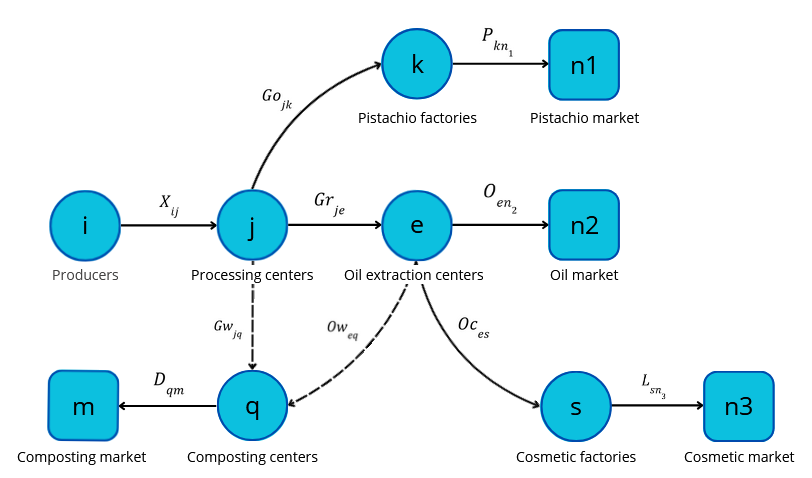
\includegraphics[width=8.4cm]{./imgs/supplychain.PNG}
      \caption{Cadeia de Suprimentos de PistacFhe proposta}
      \label{fig:supplychain}
  \end{center}
\end{figure}
    
\begin{itemize}
\item A função objetivo \eqref{eq:custo} minimiza os custos totais da cadeia de suprimentos, incluindo custos de abertura, transporte e produção. Os custos são divididos em três componentes: 
$z_1$ \eqref{eq:custo1}, $z_2$ \eqref{eq:custo2}, e $z_3$ \eqref{eq:custo3}, que representam os custos de abertura de instalações, transporte e produção, respectivamente, conforme mostrado nas seguintes equações:
\end{itemize}

\begin{align}
  z_1 &= \sum_{j=1}^J Fu_j \cdot U_j 
      + \sum_{q=1}^Q Fy_q \cdot Y_q
      + \sum_{k=1}^{K} Fw_k \cdot W_k \notag \\
      &\quad + \sum_{e=1}^{E} Fr_e \cdot R_e
      + \sum_{s=1}^S Fv_s \cdot V_s
      \label{eq:custo1}
\end{align}

\begin{align}
  z_2 &= \sum_{i=1}^I\sum_{j=1}^J CI_i \cdot X_{ij} 
      + \sum_{j=1}^J\sum_{k=1}^K Cu_{1j} \cdot Go_{jk} \notag \\
      &\quad + \sum_{j=1}^J\sum_{e=1}^E Cu_{2j} \cdot Gr_{je} 
      + \sum_{q=1}^Q\sum_{m=1}^M Cy_q \cdot D_{qm} \notag \\
      &\quad + \sum_{k=1}^K\sum_{n_1=1}^{N_1} Cw_k \cdot P_{kn_1}
      \label{eq:custo2}
\end{align}

\begin{align}
  z_3 &= \sum_{i=1}^I\sum_{j=1}^J CX_{ij} \cdot X_{ij} 
      + \sum_{j=1}^J\sum_{k=1}^K CK_{jk} \cdot Go_{jk} \notag \\
      &\quad + \sum_{j=1}^J\sum_{q=1}^Q CJ_{jq} \cdot Gw_{jq}
      + \sum_{e=1}^E\sum_{s=1}^S CS_{es} \cdot Oc_{es} \notag \\
      &\quad + \sum_{e=1}^E\sum_{q=1}^Q CQ_{eq} \cdot Ow_{eq}
      \label{eq:custo3}
\end{align}

\begin{itemize}
  \item As variáveis $R_j$, $Y_q$, $W_k$, $Z_e$ e $V_s$ são binárias e determinam se certos elementos do modelo estão ativos. Por exemplo, $R_j = 1$ indica que a instalação $j$ está operacional, e $R_j = 0$ caso contrário. As demais variáveis do modelo são contínuas e não negativas, representando valores reais maiores ou iguais a zero. Essas variáveis modelam fluxos, quantidades e outros fatores mensuráveis dentro do sistema.
  
  \item As restrições \eqref{eq:restricao1}-\eqref{eq:restricao6} tratam das limitações de capacidade e demanda de cada instalação na cadeia de suprimentos. Em particular, a restrição \eqref{eq:restricao1} limita a quantidade de produtos transportados dos produtores para os centros de distribuição. Já as restrições \eqref{eq:restricao2}-\eqref{eq:restricao6} garantem que as quantidades enviadas para os centros de processamento, compostagem, fábricas de pistache, centros de extração de óleo e fábricas de cosméticos não ultrapassem as capacidades dessas instalações.
  
  \item A quantidade de produtos enviados de qualquer instalação não deve ultrapassar os pedidos recebidos por essa instalação. Consequentemente, a restrição \eqref{eq} estabelece que a quantidade de produtos expedidos de um centro de processamento deve ser menor ou igual à quantidade recebida por outras instalações. As restrições \eqref{eq}-\eqref{eq} definem as quantidades de pistaches de casca aberta, sementes cruas e resíduos gerados durante o processo de descascamento em cada centro de processamento. De forma similar, as restrições \eqref{eq}-\eqref{eq} regem os fluxos dentro das fábricas de pistache, centros de extração de óleo, fábricas de cosméticos e centros de compostagem.
  
  \item Por fim, para garantir que a demanda dos clientes seja atendida, as restrições \eqref{eq:restricao17}-\eqref{eq:restricao20} asseguram que as quantidades de produtos entregues aos clientes de pistache, óleo de pistache, cosméticos e composto satisfaçam ou superem suas respectivas demandas.
\end{itemize}

%===============================================================================

\section{Metodologia}
\label{sec:heuristic1}

Esta seção apresenta a metodologia utilizada para resolver o problema de otimização, empregando codificação baseada em prioridade \citep{gen2006genetic} e o algoritmo de Busca em Vizinhança Variável (VNS). A codificação 
baseada em prioridade ordena as variáveis de decisão para explorar o espaço de soluções mantendo a viabilidade, enquanto a VNS alterna entre diferentes estruturas de vizinhança para escapar de ótimos locais. 
Nossa abordagem inclui operadores de vizinhança personalizados e configurações de parâmetros adequadas.

\subsection{Representação da Solução}
Seguindo \cite{rajabi2023utilizing} e \cite{gen2006genetic}, utilizamos a codificação baseada em prioridade para representar as soluções. Cada par origem-destino é tratado como um gene, cujas prioridades 
orientam a construção da árvore de transporte. O processo de decodificação seleciona iterativamente o nó de maior prioridade, conectando-o à alternativa de menor custo, garantindo sempre o cumprimento das 
restrições de viabilidade.

Diferentemente de \cite{rajabi2023utilizing}, que utiliza números reais entre 0 e 1, adotamos números inteiros de 1 a $Z$ para melhorar a interpretabilidade e facilitar as operações de vizinhança. A eficácia 
dessa codificação já foi demonstrada em otimização de cadeias de suprimentos \citep{pishvaee2010memetic,altiparmak2006genetic,liu2023integrated}.

O processo de decodificação garante a conformidade com as restrições \eqref{eq:custo}-\eqref{eq:restricao20}, determinando sequencialmente os fluxos dos produtores para os centros de processamento, fábricas e 
consumidores, minimizando os custos de transporte. Ajustes são feitos para priorizar as entidades com maior necessidade, assegurando a viabilidade. Da mesma forma, a compostagem e o gerenciamento de resíduos 
seguem restrições rigorosas de capacidade e demanda para otimizar a distribuição.

A Figura~\ref{fig:decode_flux} ilustra o processo de decodificação, que inicia com o fluxo de produtos derivados do pistache das fábricas para os consumidores, garantindo o atendimento de todas as restrições. 
Os fluxos de óleo e produtos cosméticos seguem princípios semelhantes. Os centros de processamento regulam a alocação do pistache, considerando perdas produtivas e garantindo uma distribuição viável. Os pistaches
colhidos são distribuídos proporcionalmente entre fábricas e centros de extração de óleo, priorizando o atendimento da demanda e minimizando custos de transporte. Os fluxos entre produtores e centros de 
processamento não podem exceder a capacidade de produção, garantindo a viabilidade do sistema. Os fluxos de resíduos e fertilizantes são gerenciados de forma semelhante, respeitando os limites de capacidade 
de processamento e compostagem, enquanto minimizam os custos.

\begin{figure}[h!]
  \begin{center}
  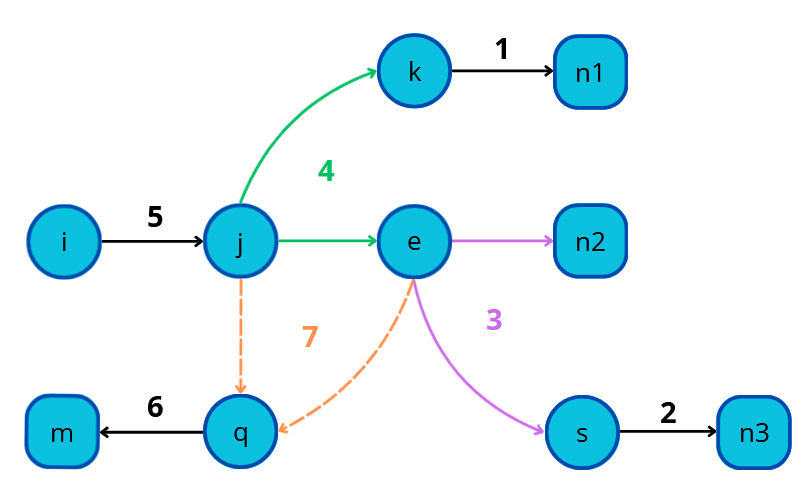
\includegraphics[width=8.4cm]{./imgs/decode_flux.PNG}
  \caption{Etapas de decodificação do fluxo de produtos na cadeia de suprimentos}
  \label{fig:decode_flux}
  \end{center}
\end{figure}

\subsection{Busca em Vizinhança Variável (VNS)}
A Busca em Vizinhança Variável (VNS) explora o espaço de soluções alterando sistematicamente as estruturas de vizinhança \citep{gendreau2010handbook}. O algoritmo alterna entre as fases de perturbação 
(\textit{shaking}) e busca local, aceitando novas soluções apenas se melhorarem a função objetivo. Essa abordagem tem se mostrado eficaz na resolução de problemas de otimização com restrições \citep{imran2009variable,fleszar2008effective,burke2010hybrid}.

A implementação do algoritmo VNS utilizado neste estudo está descrita no Algoritmo \ref{algoVNS}.

\begin{algorithm}
  \caption{Busca em Vizinhança Variável (VNS)}\label{algoVNS}
  \begin{algorithmic}[1]
  \Require Solução inicial $x$, tamanho máximo da vizinhança $k_{\text{max}}$, limite de tempo $t_{\text{max}}$
  \State \textbf{Saída:} Melhor solução encontrada $x^*$
  \State $x^ \Leftarrow x$
  \Repeat
  \State $k \Leftarrow 1$
  \Repeat
  \State $x' \Leftarrow \text{Shake}(x, k)$
  \State $x'' \Leftarrow \text{LocalSearch}(x')$
  \If{$f(x'') < f(x^)$}
  \State $x^ \Leftarrow x''$, $k \Leftarrow 1$
  \Else
  \State $k \Leftarrow k + 1$
  \EndIf
  \Until{$k > k_{\text{max}}$}
  \State $t \Leftarrow \text{CpuTime}()$
  \Until{$t > t_{\text{max}}$}
  \end{algorithmic}
\end{algorithm}

\subsection{Estruturas de Vizinhança}
Quatro operadores clássicos de vizinhança \citep{devika2014designing}, ilustrados na Figura \ref{fig:nbdh_op}, são utilizados para aumentar a diversidade das soluções:

\begin{itemize}
\item \textbf{Swap:} Permuta dois elementos no cromossomo.
\item \textbf{Reversion:} Inverte a sequência de elementos entre dois índices selecionados \citep{vahdani2010scheduling}.
\item \textbf{Insertion:} Move um elemento para uma nova posição, deslocando os demais conforme necessário \citep{rabiee2012scheduling}.
\item \textbf{Slide:} Remove um elemento, desloca os outros e o reinsere em uma nova posição.
\end{itemize}

Cada operação é aplicada a um vetor de prioridade selecionado aleatoriamente dentro do conjunto de soluções, garantindo a viabilidade e aumentando a eficiência da busca.

\begin{figure}[h!]
  \begin{center}
  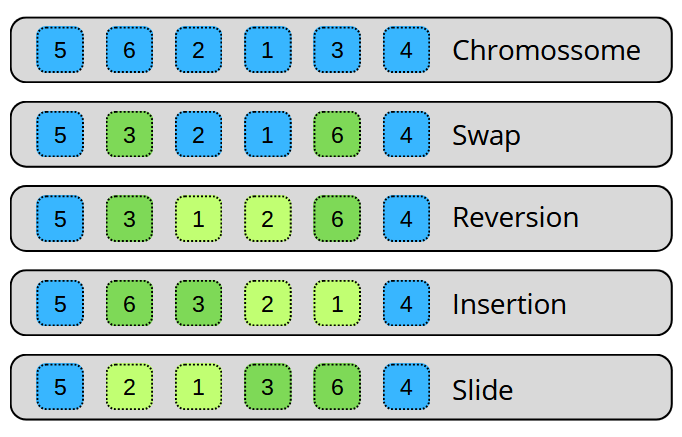
\includegraphics[width=8.4cm]{./imgs/nbhd_op.png}
  \caption{Estruturas de vizinhança utilizadas no algoritmo VNS}
  \label{fig:nbdh_op}
  \end{center}
\end{figure}

%===============================================================================

\section{Experimentos Computacionais}
\label{sec:experiments1}

O método heurístico proposto foi testado em instâncias de diferentes tamanhos, definidos pelo número de elementos em cada entidade do problema ($I$, $J$, $K$, $E$, $S$, $Q$, $N_1$, $N_2$, $N_3$ e $M$).
Os tamanhos testados foram 100, 200, 400, 800 e 1600, resultando em contagens totais de variáveis de 100.500; 401.000; 1.602.000; 6.404.000; e 25.608.000, respectivamente.
Entretanto, algoritmos que utilizam codificação baseada em prioridade possuem um número significativamente menor de variáveis, pois consideram apenas as prioridades dos pares fonte-depósito.
Nesses casos, as contagens de variáveis foram reduzidas para 1.700; 3.400; 6.800; 13.600; e 27.200.

Os parâmetros das instâncias, como capacidades e demandas, foram gerados aleatoriamente conforme a Tabela 7 de \cite{rajabi2023utilizing}. A abordagem baseada em VNS foi comparada com um Algoritmo Genético (GA),
que foi uma das meta-heurísticas evolucionárias utilizadas na referência considerada. O GA utilizou mutações baseadas em troca (\textit{swap-based mutations}) e cruzamentos de subsequências (\textit{subsequence-exchanging crossovers}),
com vetores selecionados aleatoriamente, uma população de 100 indivíduos e uma estratégia de seleção por Torneio Binário.

Tanto o VNS quanto o GA foram executados 30 vezes por instância, com um critério de parada de 100.000 avaliações da função objetivo. Os experimentos foram conduzidos em um sistema com Ubuntu 24.04.1 LTS,
processador Intel Xeon E3-1240 V2 (8 núcleos) e 32 GB de RAM.

\subsection{Comparação entre VNS e GA}

A comparação com o GA segue a metodologia de \cite{rajabi2023utilizing}, embora uma correspondência exata não tenha sido possível devido às diferenças no processo de decodificação.
A Tabela \ref{tab:comparison_vns_ga} apresenta o desempenho médio das 30 melhores soluções obtidas por cada algoritmo. Para instâncias pequenas (100 elementos), VNS e GA apresentaram desempenho semelhante,
com uma melhoria de apenas 0,71\% para o VNS. No entanto, em instâncias maiores, o VNS superou consistentemente o GA, alcançando melhorias entre 3,4\% e 5,3\%.

Os boxplots na Fig. \ref{fig:VNSxGA_boxplots} ilustram a distribuição das soluções, destacando diferenças significativas nos casos de 800 e 1600 instâncias. Os valores de p obtidos no teste t para amostras 
independentes (teste de Welch) para essas instâncias são inferiores a 0,05, indicando que as diferenças observadas são estatisticamente significativas, considerando normalidade e variâncias desiguais. 
Esses resultados sugerem que o VNS tem um desempenho significativamente superior ao GA em problemas de grande escala do ponto de vista estatístico. Além disso, o GA apresentou tempos de execução mais 
longos, provavelmente devido ao aumento dos custos computacionais de suas operações evolutivas à medida que o tamanho do problema crescia.

Em resumo, embora o GA tenha um desempenho competitivo em instâncias pequenas, sua escalabilidade é limitada. Em contraste, o VNS não apenas obtém soluções superiores,
mas também demonstra maior eficiência no tratamento de problemas de grande escala, estabelecendo-se como um método de otimização mais robusto e escalável.

\begin{figure*}[h!]
  \centering
  \begin{tabular}{cc}
      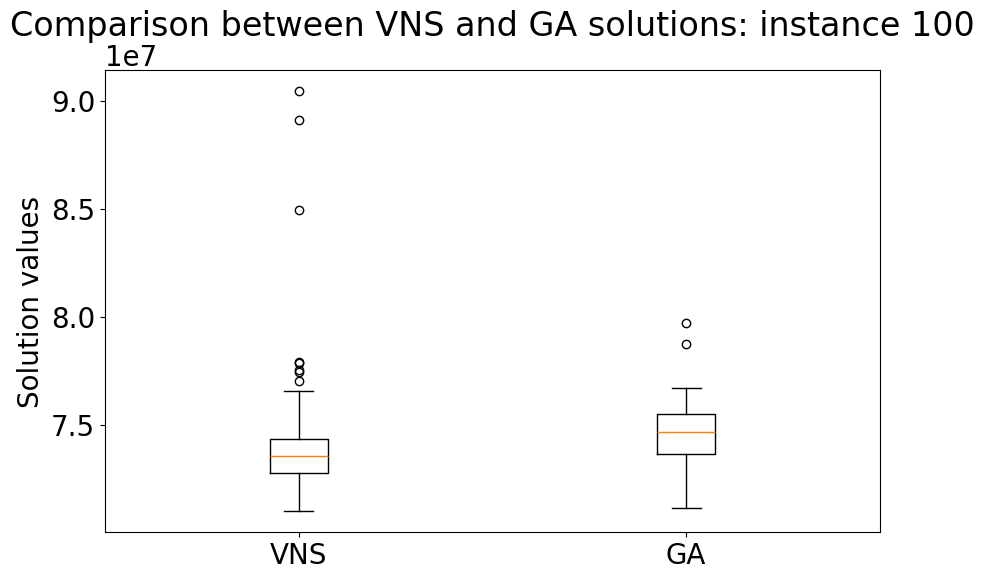
\includegraphics[width=0.45\textwidth]{./imgs/VNSxGA_100.png} & 
      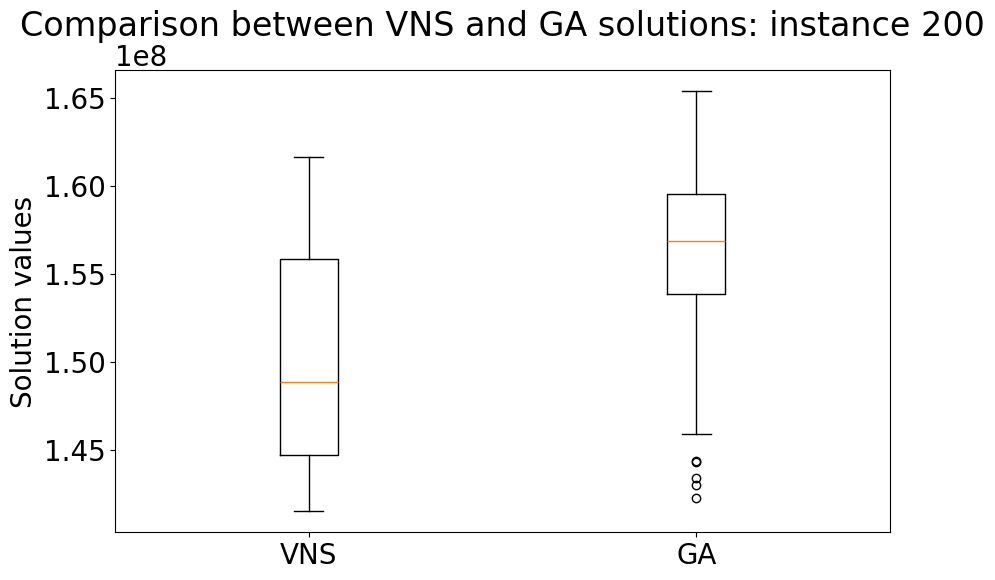
\includegraphics[width=0.46\textwidth]{./imgs/VNSxGA_200.png} \\
      (a) $I, J, K, E, S, Q, N1, N2, N3, M = 100$ & 
      (b) $I, J, K, E, S, Q, N1, N2, N3, M = 200$ \\
      \vspace{0.5cm} \\ % Adds vertical space
      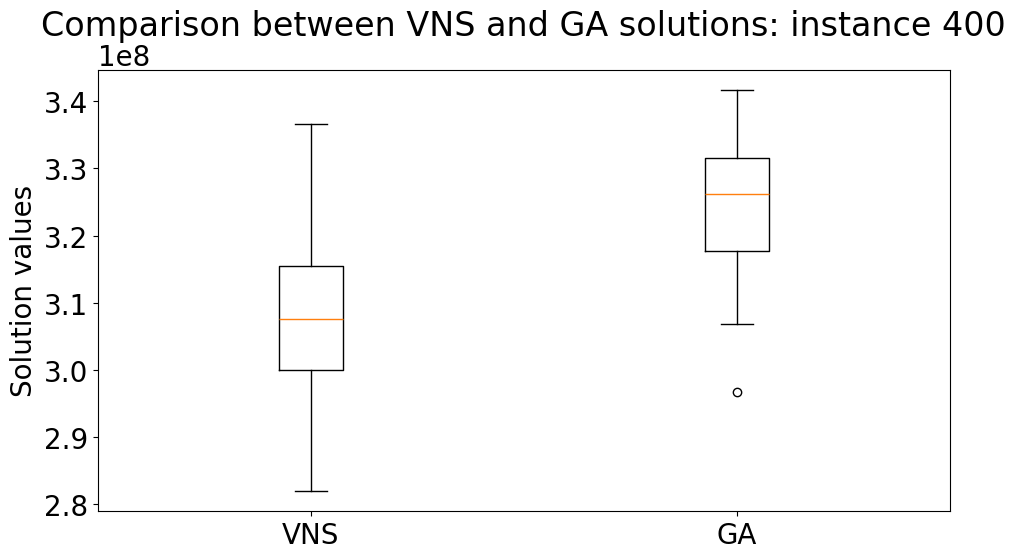
\includegraphics[width=0.47\textwidth]{./imgs/VNSxGA_400.png} & 
      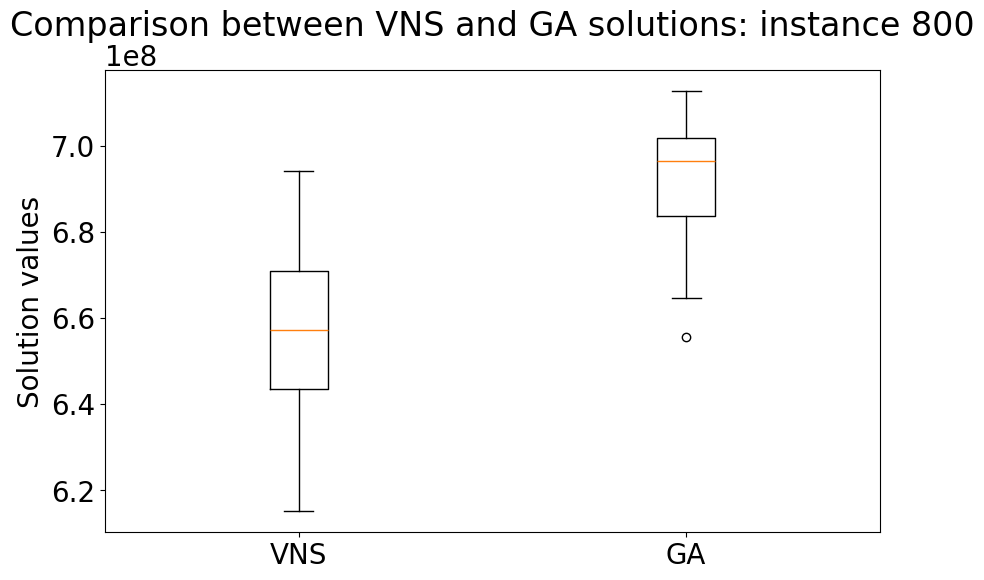
\includegraphics[width=0.45\textwidth]{./imgs/VNSxGA_800.png} \\
      (c) $I, J, K, E, S, Q, N1, N2, N3, M = 400$ & 
      (d) $I, J, K, E, S, Q, N1, N2, N3, M = 800$ \\
      \vspace{0.5cm} \\ % Adds vertical space
      \multicolumn{2}{c}{
          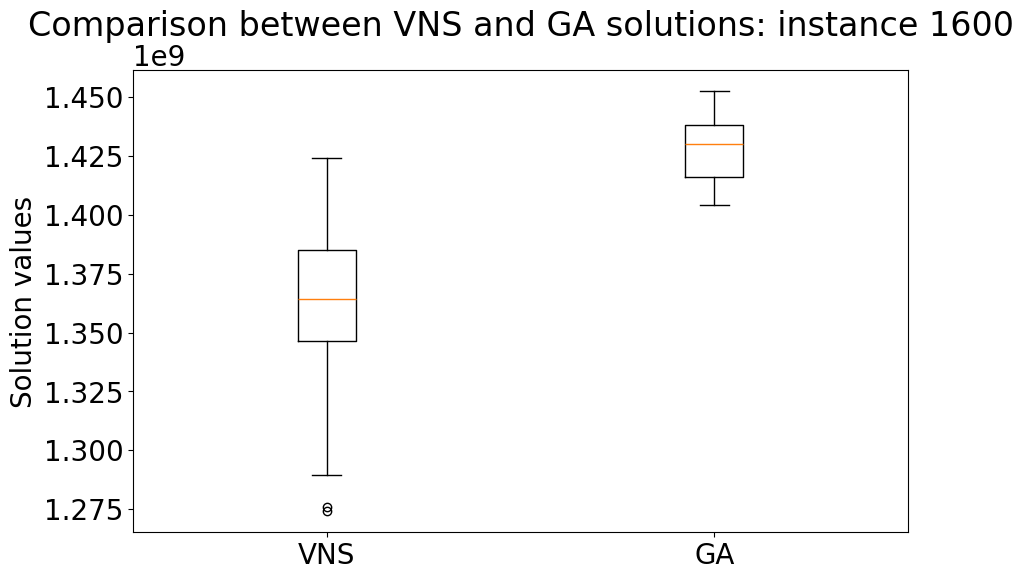
\includegraphics[width=0.45\textwidth]{./imgs/VNSxGA_1600.png} 
      } \\
      \multicolumn{2}{c}{(e) $I, J, K, E, S, Q, N1, N2, N3, M = 1600$} \\
  \end{tabular}
  \caption{Boxplots comparando o desempenho do algoritmo VNS e de uma meta-heurística baseada em população (Algoritmo Genético) em diferentes tamanhos de problema, com base nos valores da função objetivo.}
  \label{fig:VNSxGA_boxplots}
\end{figure*}

% \begin{table}[hb]
%   \begin{center}
%   \caption{Comparison of the VNS algorithm and a population-based metaheuristic (genetic algorithm) in terms of the average objective function value of the best solutions and the average execution time.}
%   \label{tab:comparison_vns_ga}
%   \begin{tabular}{cccc}
%   \hline
%   Instance & VNS & GA & Difference (\%) \\ \hline
%   100  & $7.41 \times 10^7$  & $7.46 \times 10^7$  & 0.71 \\  
%   200  & $1.50 \times 10^8$  & $1.55 \times 10^8$  & 3.37 \\  
%   400  & $3.08 \times 10^8$  & $3.24 \times 10^8$  & 5.31 \\  
%   800  & $6.57 \times 10^8$  & $6.92 \times 10^8$  & 5.26 \\  
%   1600 & $1.36 \times 10^9$  & $1.43 \times 10^9$  & 4.64 \\ \hline
%   \end{tabular}
%   \end{center}
% \end{table}

\begin{table*}[!htb]
  \caption{Comparação entre o algoritmo VNS e uma meta-heurística baseada em população (Algoritmo Genético) em termos do valor médio da função objetivo das melhores soluções e do tempo médio de execução.}
  \label{tab:comparison_vns_ga}
  \begin{tabular*}{\textwidth}{@{\extracolsep\fill}lccccc}
  \toprule%
  & \multicolumn{3}{@{}c@{}}{Avaliação da função objetivo (média)} & \multicolumn{2}{@{}c@{}}{Tempo de Execução (média)} \\\cmidrule{2-4}\cmidrule{5-6}%
  Instância & VNS & GA & Diferença (\%) & VNS & GA \\
  \midrule
  100  & $7.41 \times 10^6$  & $7.46 \times 10^6$  & 0.71 & 241s  & 6,595s \\
  200  & $1.50 \times 10^8$  & $1.55 \times 10^8$  & 3.37 & 714s  & 14,349s \\
  400  & $3.08 \times 10^8$  & $3.24 \times 10^8$  & 5.31 & 2,016s & 33,941s \\
  800  & $6.57 \times 10^8$  & $6.92 \times 10^8$  & 5.26 & 5,538s & 82,687s \\
  1600 & $1.36 \times 10^9$  & $1.43 \times 10^9$  & 4.64 & 17,767s & 217,958s \\
  \bottomrule 
  \end{tabular*}
\end{table*}

%===============================================================================
\section{Conclusão}
\label{sec:conclusion1}

Este estudo apresenta um modelo de otimização para a cadeia de suprimentos de pistache, abordando as complexidades do gerenciamento de produtos e subprodutos ao longo de múltiplas etapas. 
Ao integrar produção, transporte e operações das instalações, o modelo garante uma alocação eficiente de recursos, respeitando as restrições de capacidade e demanda. Formulado como um problema 
de Programação Linear Inteira Mista (MILP), ele é resolvido por meio do algoritmo Variable Neighborhood Search (VNS), que explora o espaço de soluções utilizando estruturas de vizinhança como 
Swap, Reversion, Insertion e Slide.

A análise comparativa demonstra a superioridade do VNS em relação aos Algoritmo Genético (GA), tanto em qualidade das soluções quanto em eficiência computacional, especialmente para 
instâncias de grande escala, onde métodos exatos se tornam inviáveis devido a limitações de tempo e memória.

Pesquisas futuras podem explorar operadores de vizinhança específicos para o problema, aprimorando ainda mais o desempenho do VNS. Além disso, uma abordagem híbrida, combinando VNS com métodos 
exatos, pode melhorar tanto a precisão quanto a eficiência da solução, tornando a metodologia mais aplicável a diferentes setores.

O código e conjunto de dados utilizados neste estudo estão disponíveis em: \url{https://github.com/raissagd/Pistachio_CLSC}.

\else
% ===============================================================
% ===============================================================
% USE THIS PART IF THE TEXT IS IN ENGLISH
% ===============================================================
% ===============================================================
% 

\begin{frontmatter}

\title{Optimizing Pistachio Supply Chains with Enhanced Metaheuristics}

\author[First]{Raissa Gon\c{c}alves Diniz} 
\author[Second]{Andr\'e Costa Batista} 

\address[First]{Operations Research and Complex Systems Laboratory, Universidade Federal de Minas Gerais, Brazil (e-mail: raissagd@ufmg.br).}
\address[Second]{Department of Electrical Engineering, Universidade Federal de Minas Gerais, Av. Ant\^onio Carlos 6627, Belo Horizonte, 31270-010, Minas Gerais, Brazil (e-mail: andre-costa@ufmg.br).}

\renewcommand{\abstractname}{{\bf Abstract:~}}   

\begin{abstract}                
Supply chains play a crucial role in the agricultural industry, especially for high-value crops such as pistachios, where effective management can drive economic growth and promote sustainability. While previous research has explored optimization strategies for pistachio supply chains, the majority of these studies predominantly rely on population-based algorithms to tackle these challenges. In this work, we introduce the use of a Variable Neighborhood Search (VNS) algorithm and evaluate its performance in comparison to a population-based metaheuristic, specifically the Genetic Algorithm (GA). The results indicate that VNS consistently achieves better performance than GA, both in terms of computational efficiency and solution quality, particularly for larger problem instances. As a result, the proposed method demonstrates to be an effective approach for addressing supply chain optimization problems.
\end{abstract}

\begin{keyword}
Supply Chain Optimization, Metaheuristics, Variable Neighborhood Search, Sustainability
\end{keyword}

\end{frontmatter}

%===============================================================================
%===============================================================================
%===============================================================================


\section{Introduction}
\label{sec:intro}
Agriculture plays a crucial role in economic development, contributing not only to food security but also to exports and industrial growth. Among high-value crops, 
pistachios are particularly significant in international trade, with the US, Turkey, and Iran leading global production \citep{statista2023pistachio}. Efficient supply chain management is essential 
to maintaining product quality, reducing environmental impact, and ensuring effective distribution. One key challenge in pistachio production is handling by-products 
such as hulls and shells, which, if mismanaged, can degrade soil quality and pose health risks due to mold-induced aflatoxin contamination \citep{dronavalli2019}. 
Sustainable waste management strategies, such as composting and biogas production, have been explored to mitigate these issues, as discussed by \cite{cheraghalipour2022bi}.

Supply chain inefficiencies can impact both product quality and trade. Prior studies, such as \cite{rajabi2023utilizing}, have explored optimization 
techniques using Genetic Algorithms (GA) and other evolutionary metaheuristics for pistachio logistics. However, these comparisons often rely on best-found solutions without 
strong statistical validation of superior performance. Additionally, debates persist on whether differences in bio-inspired metaheuristics significantly affect solution quality.

Building upon this foundation, this study aims to optimize pistachio supply chains using Variable Neighborhood Search (VNS), a heuristic well-suited for large 
combinatorial problems with minimal parameter tuning. We address the mixed linear model proposed in \cite{rajabi2023utilizing} for forward and reverse logistics, 
incorporating by-product reuse to minimize costs and environmental impact. Our results demonstrate that VNS outperforms GA in objective function evaluation while 
achieving competitive solutions with significantly lower computational time compared to an exact method.

The remainder of this paper is structured as follows: Section~\ref{sec:problem-def} defines the problem, describing the supply chain network and optimization objectives. Section~\ref{sec:heuristic} presents 
the heuristic approach, detailing the VNS methodology and its implementation. Section~\ref{sec:experiments} compares experimental results between VNS and GA. Finally, Section~\ref{sec:conclusion}
concludes with key findings and future research directions.


%===============================================================================


\section{Problem Definition}
\label{sec:problem-def}

The network proposed by \cite{rajabi2023utilizing}, as depicted in Figure \ref{fig:supplychain}, consists of producers, processing centers, pistachio factories, oil extraction centers, composting centers, and customers. Pistachios are transported from orchards to processing centers, where they are processed into open-mouth pistachios, raw kernels, and waste. These outputs are then sent to factories, oil extraction centers, and composting centers, respectively. Open-mouth pistachios are roasted, packaged, and delivered to customers, while pistachio oil is supplied to oil customers and cosmetic factories. Waste is converted into compost for distribution. Although the compost is returned to the producers, ideally creating a closed-loop system, the mathematical model does not establish a direct connection between the compost customers and the producers who supply pistachios to the processing centers. Strictly speaking, the mathematical flow model does not implement a closed-loop. Instead, it interprets the flow of compost to its respective customers as feedback, even though these customers are not necessarily linked to the variables associated with the producers. Similar approaches have been adopted in other studies \citep{pishvaee2010memetic,ahmadi2019integrated,banasik2016simple}, and the strict implementation of a feedback loop could be a promising direction for future research.

The mixed-integer linear problem aims to minimize total costs \eqref{eq:custo}, including opening, transportation, production costs, under the following capacity and demand constraints 
with no allowed shortages (see further details regarding the variables in the Table 5 of \cite{rajabi2023utilizing}):
    
\begin{align}
    \min &\ z_1 + z_2 + z_3 \label{eq:custo}\\
    \text{s.t.:} \quad & \sum\limits_{j=1}^J X_{ij} \le Cpa_i, \quad \forall i \in I \label{eq:restricao1}\\
    & \sum\limits_{i=1}^I X_{ij} \le Cpu_j\times U_j, \quad \forall j \in J \label{eq:restricao2}\\
    & \sum\limits_{e=1}^E Ow_{eq} + \sum\limits_{j=1}^J Gw_{jq} \le Cpy_q \times Y_q, \quad \forall q \in Q \label{eq:restricao3}\\
    & \sum\limits_{j=1}^J Go_{jk} \le Cpw_k\times W_k, \quad \forall k \in K \label{eq:restricao4}\\
    & \sum\limits_{j=1}^J Gr_{je} \le Cpr_e\times R_e, \quad \forall e \in E \label{eq:restricao5}\\
    & \sum\limits_{e=1}^E O_{en_2} \le Cpv_s\times V_s, \quad \forall s \in S \label{eq:restricao6}\\
    & \sum\limits_{k=1}^K Go_{jk} + \sum\limits_{e=1} Gr_{je} + \sum\limits_{q=1}^Q Gw_{jq} \le \sum\limits_{i=1} X_{ij}, \quad \forall j \in J \label{eq:restricao7} \\
    & \sum\limits_{k=1}^K Go_{jk} = (1-\beta) \sum\limits_{i=1}^I X_{ij}\theta_1, \quad \forall j\in J \label{eq:restricao8}\\
    & \sum\limits_{e=1}^K Gr_{je} = (1-\beta) \sum\limits_{i=1}^I X_{ij}\theta_2, \quad \forall j\in J \label{eq:restricao9}\\
    & \sum\limits_{q=1}^Q Gw_{jq} = \sum\limits_{i=1}^I X_{ij}\theta_3, \quad \forall j\in J \label{eq:restricao10}\\
    & \theta_1 + \theta_2 + \theta_3 = 1 \label{eq:restricao11} \\
    & \sum\limits_{n_1=1}^{N_1} P_{kn_1} \le \sum\limits_{j=1}^J Go_{jk} \times \gamma k, \quad \forall k \in K \label{eq:restricao12}\\
    & \sum\limits_{n_2=1}^{N_2} O_{en_2} + \sum\limits_{s=1}^S Oc_{es} \le \sum\limits_{j=1} Gr_{je}\times(1-\lambda), \quad \forall e\in E \label{eq:restricao13}\\
    & \sum\limits_{q=1}^{Q} Ow_{eq} \le \sum\limits_{j=1}^J Gr_{je} \times \lambda, \quad \forall e \in E \label{eq:restricao14}\\
    & \sum\limits_{n_3=1}^{N_3} L_{sn_1} \le \sum\limits_{e=1}^E Oc_{es} \times \gamma s, \quad \forall s \in S \label{eq:restricao15}
\end{align}
\begin{align}
  & \sum\limits_{m=1}^M D_{qm} \le \left(\sum\limits_{j=1}^J Gw_{jq} + \sum\limits_{e=1}^E Ow_{eq} \right) \times \gamma q, \quad \forall q \in Q \label{eq:restricao16}\\
  & \sum\limits_{k=1}^K P_{kn_1} \ge Dp_{n_1}, \quad \forall n_1 \in N_1 \label{eq:restricao17}\\
  & \sum\limits_{e=1}^E O_{en_2} \ge Du_{n_2}, \quad \forall n_2 \in N_2 \label{eq:restricao18}\\
  & \sum\limits_{s=1}^S L_{sn_3} \ge Ds_{n_3}, \quad \forall n_3 \in N_3 \label{eq:restricao19}\\
  & \sum\limits_{q=1}^Q D_{qm} \le Dc_{m}, \quad \forall m \in M \label{eq:restricao20}
\end{align}

\begin{figure}
  \begin{center}
      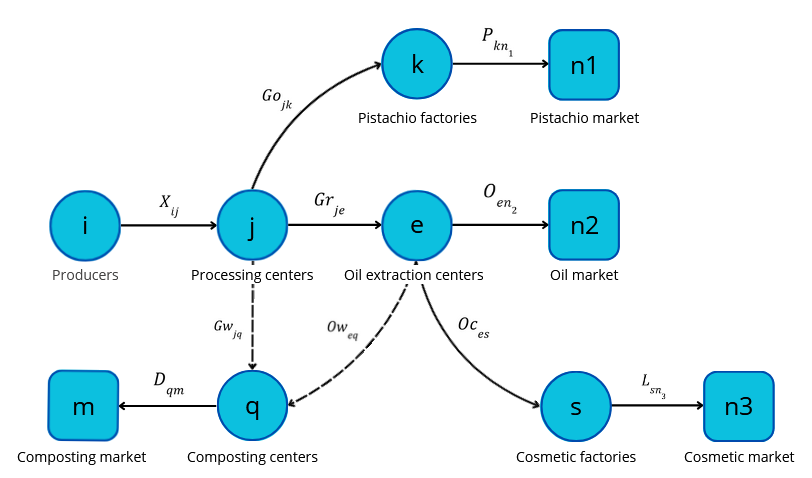
\includegraphics[width=8.4cm]{./imgs/supplychain.PNG}
      \caption{Proposed pistachio supply chain network}
      \label{fig:supplychain}
  \end{center}
\end{figure}
    
\begin{itemize}
\item The objective function \eqref{eq:custo} minimizes the total costs of the supply chain, including opening, transportation, and production costs. The costs are divided into three components: 
$z_1$ \eqref{eq:custo1}, $z_2$ \eqref{eq:custo2}, and $z_3$ \eqref{eq:custo3}, which represent the costs of opening facilities, transportation, and production, respectively as shown in the following equations:
\end{itemize}

\begin{align}
  z_1 &= \sum_{j=1}^J Fu_j \cdot U_j 
      + \sum_{q=1}^Q Fy_q \cdot Y_q
      + \sum_{k=1}^{K} Fw_k \cdot W_k \notag \\
      &\quad + \sum_{e=1}^{E} Fr_e \cdot R_e
      + \sum_{s=1}^S Fv_s \cdot V_s
      \label{eq:custo1}
\end{align}

\begin{align}
  z_2 &= \sum_{i=1}^I\sum_{j=1}^J CI_i \cdot X_{ij} 
      + \sum_{j=1}^J\sum_{k=1}^K Cu_{1j} \cdot Go_{jk} \notag \\
      &\quad + \sum_{j=1}^J\sum_{e=1}^E Cu_{2j} \cdot Gr_{je} 
      + \sum_{q=1}^Q\sum_{m=1}^M Cy_q \cdot D_{qm} \notag \\
      &\quad + \sum_{k=1}^K\sum_{n_1=1}^{N_1} Cw_k \cdot P_{kn_1}
      \label{eq:custo2}
\end{align}

\begin{align}
  z_3 &= \sum_{i=1}^I\sum_{j=1}^J CX_{ij} \cdot X_{ij} 
      + \sum_{j=1}^J\sum_{k=1}^K CK_{jk} \cdot Go_{jk} \notag \\
      &\quad + \sum_{j=1}^J\sum_{q=1}^Q CJ_{jq} \cdot Gw_{jq}
      + \sum_{e=1}^E\sum_{s=1}^S CS_{es} \cdot Oc_{es} \notag \\
      &\quad + \sum_{e=1}^E\sum_{q=1}^Q CQ_{eq} \cdot Ow_{eq}
      \label{eq:custo3}
\end{align}

\begin{itemize}
  \item The variables $R_j$, $Y_q$, $W_k$, $Z_e$, and $V_s$ are binary decision variables that determine whether specific elements in the model are active. For instance, $R_j = 1$ indicates that facility $j$ is operational, and $R_j = 0$ otherwise. The remaining variables in the model are continuous and non-negative, representing real values greater than or equal to zero. These variables are used to model flows, quantities, and other measurable factors within the system.
  
  \item Constraints \eqref{eq:restricao1}-\eqref{eq:restricao6} address the capacity and demand limitations of each facility in the supply chain. Specifically, constraint \eqref{eq:restricao1} restricts the amount of products transported from producers to distribution centers. Constraints \eqref{eq:restricao2}-\eqref{eq:restricao6} ensure that the quantities of products sent to processing centers, composting centers, pistachio factories, oil extraction centers, and cosmetic factories do not exceed the capacities of these facilities.
  
  \item The quantity of products shipped from any facility must not surpass the orders received by that facility. Accordingly, constraint \eqref{eq:restricao7} states that the amount of products dispatched from a processing center must be less than or equal to the quantity received by other facilities. Constraints \eqref{eq:restricao8}-\eqref{eq:restricao11} define the quantities of open-mouth pistachios, raw kernels, and waste generated during the dehulling process at each processing center. Similarly, constraints \eqref{eq:restricao12}-\eqref{eq:restricao16} govern the flows within pistachio factories, oil extraction centers, cosmetic factories, and composting centers.
  
  \item Finally, to ensure that customer demand is satisfied, constraints \eqref{eq:restricao17}-\eqref{eq:restricao20} ensure that the quantities of products delivered to pistachio customers, pistachio oil customers, cosmetic customers, and compost markets meet or exceed their respective demands.
\end{itemize}

%===============================================================================

\section{Heuristic approach}
\label{sec:heuristic}

This section presents the methodology for solving the optimization problem using priority-based encoding \citep{gen2006genetic} and VNS. Priority-based encoding ranks decision variables to explore 
the solution space while maintaining feasibility, while VNS shifts between neighborhood structures to escape local optima. The approach includes tailored neighborhood operators and parameter configurations.

\subsection{Solution Representation}
Following \cite{rajabi2023utilizing} and \cite{gen2006genetic}, we employ priority-based encoding to represent solutions. Each source-depot pair is treated as a gene, with priorities guiding 
the construction of the transportation tree. The decoding process iteratively selects the highest-priority node, connecting it to the lowest-cost counterpart while ensuring feasibility constraints are met.

Unlike \cite{rajabi2023utilizing}, which uses real numbers between 0 and 1, we use integers from 1 to $Z$ to enhance interpretability and facilitate neighborhood operations. The effectiveness 
of this encoding has been already demonstrated in supply chain optimization \citep{pishvaee2010memetic,altiparmak2006genetic,liu2023integrated}.

The decoding process ensures compliance with constraints \eqref{eq:custo}-\eqref{eq:restricao20} by sequentially determining flows from producers to processing centers, factories, and consumers 
while minimizing transportation costs. Adjustments prioritize entities with the greatest need, maintaining feasibility. Similarly, composting and waste management follow strict capacity and demand 
constraints to optimize distribution.

Figure~\ref{fig:decode_flux} illustrates the decoding process, which begins with pistachio product flow from factories to consumers, ensuring all constraints are met. 
Oil and cosmetic product flows follow similar principles. Processing centers regulate pistachio allocation, considering production losses and ensuring feasible distribution. 
Harvested pistachios are proportionally allocated to factories and oil extraction centers, prioritizing demand fulfillment while minimizing transportation costs. 
Producer-to-processing center flows must not exceed production capacity, ensuring feasibility. Waste and fertilizer flows are managed similarly, respecting processing and composting capacity limits 
while minimizing costs.

\begin{figure}[h!]
  \begin{center}
  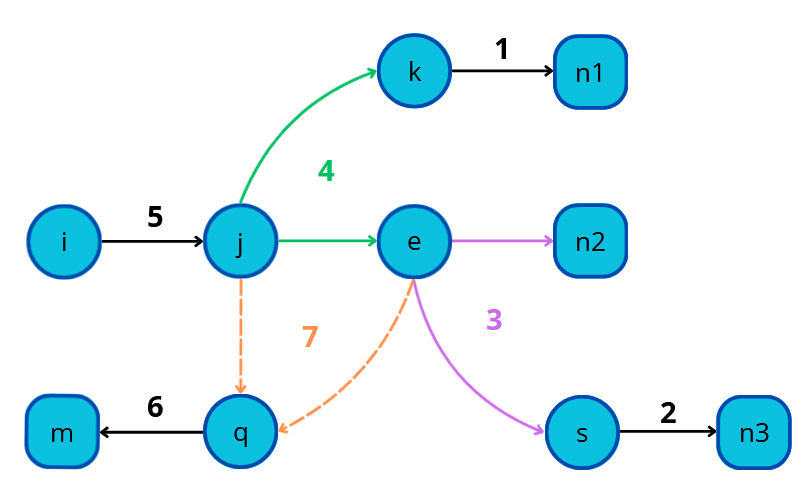
\includegraphics[width=8.4cm]{./imgs/decode_flux.PNG}
  \caption{Decodification steps of the transportation tree}
  \label{fig:decode_flux}
  \end{center}
\end{figure}

\subsection{Variable Neighborhood Search (VNS)}
VNS explores the solution space by systematically altering neighborhood structures \citep{gendreau2010handbook}. It iterates through shaking and local search phases, accepting new solutions only if 
they improve the objective function. This approach has been effective in solving constrained optimization problems \citep{imran2009variable,fleszar2008effective,burke2010hybrid}.

The implementation of the VNS algorithm used in this study is outlined in Algorithm \ref{algoVNS}.

\begin{algorithm}
\caption{Variable Neighborhood Search (VNS)}\label{algoVNS}
\begin{algorithmic}[1]
\Require Initial solution $x$, max neighborhood size $k_{\text{max}}$, time limit $t_{\text{max}}$
\State \textbf{Output:} Best solution $x^*$
\State $x^ \Leftarrow x$
\Repeat
\State $k \Leftarrow 1$
\Repeat
\State $x' \Leftarrow \text{Shake}(x, k)$
\State $x'' \Leftarrow \text{LocalSearch}(x')$
\If{$f(x'') < f(x^)$}
\State $x^ \Leftarrow x''$, $k \Leftarrow 1$
\Else
\State $k \Leftarrow k + 1$
\EndIf
\Until{$k > k_{\text{max}}$}
\State $t \Leftarrow \text{CpuTime}()$
\Until{$t > t_{\text{max}}$}
\end{algorithmic}
\end{algorithm}

\subsection{Neighborhood Structures}
Four classic neighborhood operators \citep{devika2014designing}, illustraed in Figure \ref{fig:nbdh_op}, enhance solution diversity:
\begin{itemize}
\item \textbf{Swap:} Exchanges two elements in the chromosome.
\item \textbf{Reversion:} Reverses a sequence between two selected indices \citep{vahdani2010scheduling}.
\item \textbf{Insertion:} Moves an element to a new position, shifting others accordingly \citep{rabiee2012scheduling}.
\item \textbf{Slide:} Removes an element, shifts others, and reinserts it at a new position.
\end{itemize}

Each operation is applied to a randomly selected priority vector within the solution set, maintaining feasibility and enhancing search efficiency.

\begin{figure}[h!]
  \begin{center}
  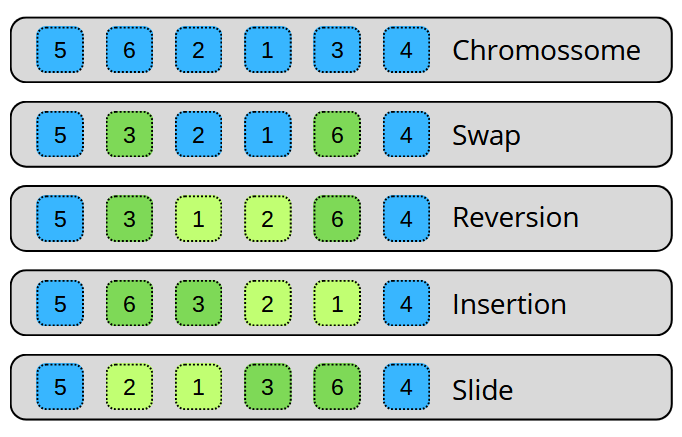
\includegraphics[width=8.4cm]{./imgs/nbhd_op.png}
  \caption{Neighborhood structures used in the VNS Algorithm}
  \label{fig:nbdh_op}
  \end{center}
\end{figure}

%===============================================================================
\section{Computational Experiments}
\label{sec:experiments}

The proposed heuristic method was tested on instances of varying sizes, defined by the number of elements in each problem entity ($I$, $J$, $K$, $E$, $S$, $Q$, $N_1$, $N_2$, $N_3$, and $M$). 
The tested sizes were 100, 200, 400, 800, and 1600, leading to total variable counts of 100,500; 401,000; 1,602,000; 6,404,000; and 25,608,000, respectively. 
However, algorithms using priority-based encoding have significantly fewer variables, as they only sum the priorities of source-depot pairs. In these cases, 
the variable counts were reduced to 1,700; 3,400; 6,800; 13,600; and 27,200.

Instance parameters, such as capacities and demands, were randomly generated following Table 7 in \cite{rajabi2023utilizing}. The proposed VNS-based approach was compared against a 
Genetic Algorithm (GA), which was one of the evolutionary algorithms used in the considered reference. The GA utilized swap-based mutations and 
subsequence-exchanging crossovers, with randomly selected vectors, a population size of 100, and a Binary Tournament selection strategy.

Both VNS and GA were run 30 times per instance, with a stopping criterion of 100,000 evaluations. Experiments were conducted on a system with Ubuntu 24.04.1 LTS, 
an Intel Xeon E3-1240 V2 (8 cores), and 32 GB RAM.

\subsection{Comparison between VNS and GA}

The comparison with GA aligns with methodologies from \cite{rajabi2023utilizing}, though an exact match was infeasible due to differences in decoding.
Table \ref{tab:comparison_vns_ga} presents the average performance of the 30 best solutions for each algorithm. For small instances (100 entities), VNS and GA performed similarly, with only 
a 0.71\% improvement in VNS. However, for larger instances, VNS consistently outperformed GA, achieving improvements between 3.4\% and 5.3\%. 

Boxplots in Fig. \ref{fig:VNSxGA_boxplots} illustrate solution distributions, showing significant differences in the 800 and 1600-instance cases. The p-values obtained from the Independent Samples T-test (Welch Test) for these instances are below 0.05, demonstrating that the observed differences are statistically significant, assuming normality and unequal variances. These findings suggest that VNS performs significantly better than GA for large-scale problems from a statistical standpoint. Additionally, GA had longer execution times, likely due to increased computational costs of its evolutionary operations as 
problem size grew.

In summary, although GA performs comparably in small-scale instances, its scalability is limited. In contrast, VNS consistently delivers better solutions and demonstrates greater efficiency in handling larger problems, establishing it as a more robust and scalable optimization method.

\begin{figure*}[h!]
  \centering
  \begin{tabular}{cc}
      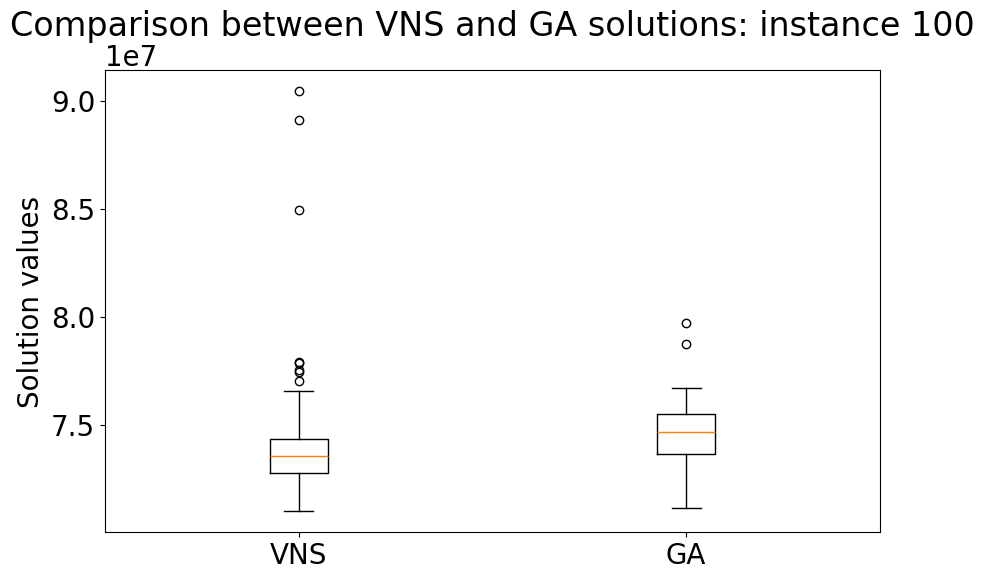
\includegraphics[width=0.45\textwidth]{./imgs/VNSxGA_100.png} & 
      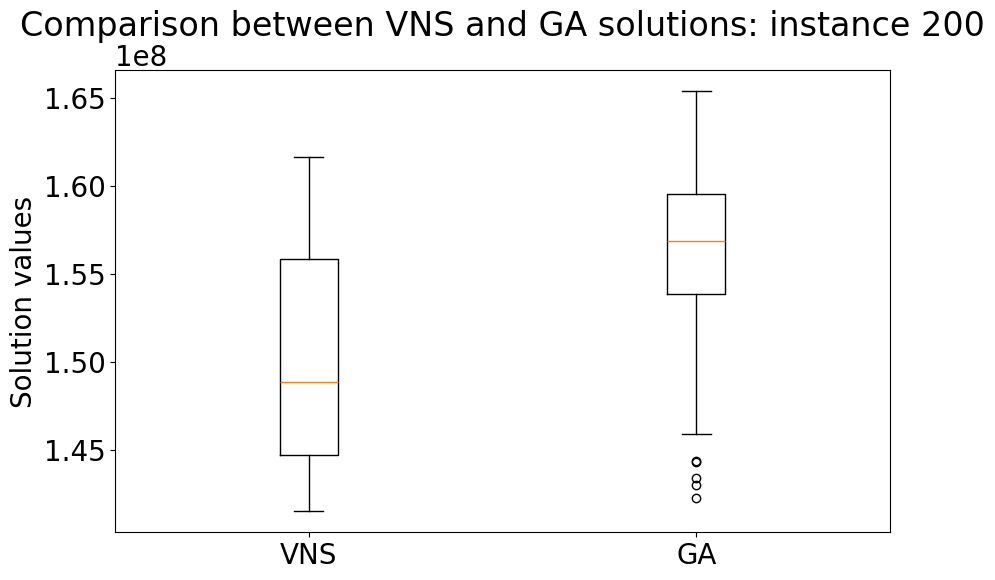
\includegraphics[width=0.46\textwidth]{./imgs/VNSxGA_200.png} \\
      (a) $I, J, K, E, S, Q, N1, N2, N3, M = 100$ & 
      (b) $I, J, K, E, S, Q, N1, N2, N3, M = 200$ \\
      \vspace{0.5cm} \\ % Adds vertical space
      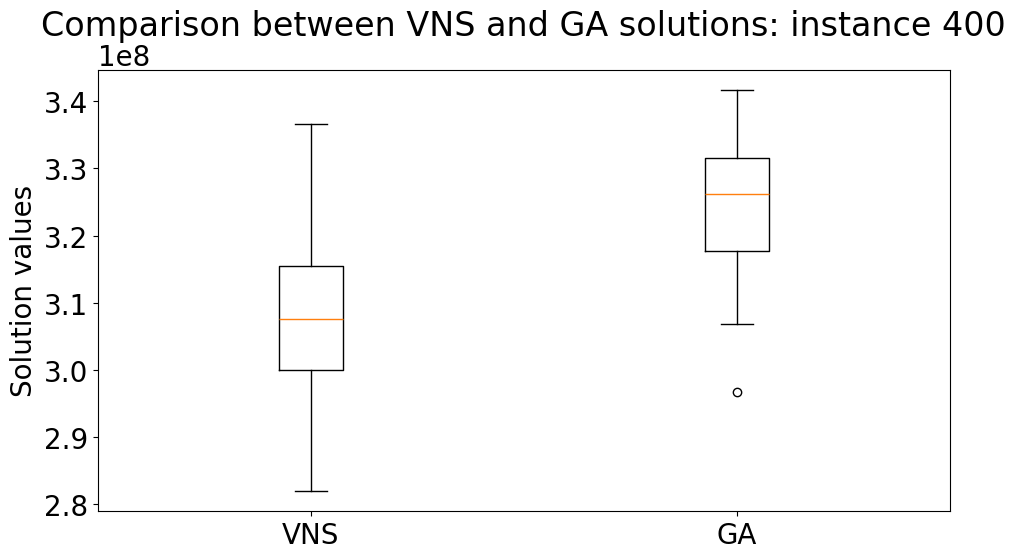
\includegraphics[width=0.47\textwidth]{./imgs/VNSxGA_400.png} & 
      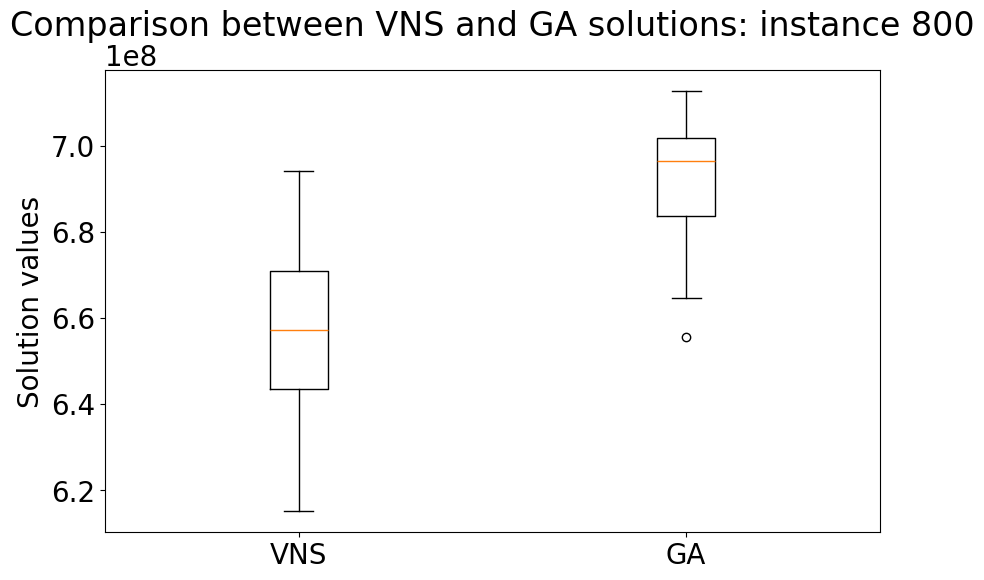
\includegraphics[width=0.45\textwidth]{./imgs/VNSxGA_800.png} \\
      (c) $I, J, K, E, S, Q, N1, N2, N3, M = 400$ & 
      (d) $I, J, K, E, S, Q, N1, N2, N3, M = 800$ \\
      \vspace{0.5cm} \\ % Adds vertical space
      \multicolumn{2}{c}{
          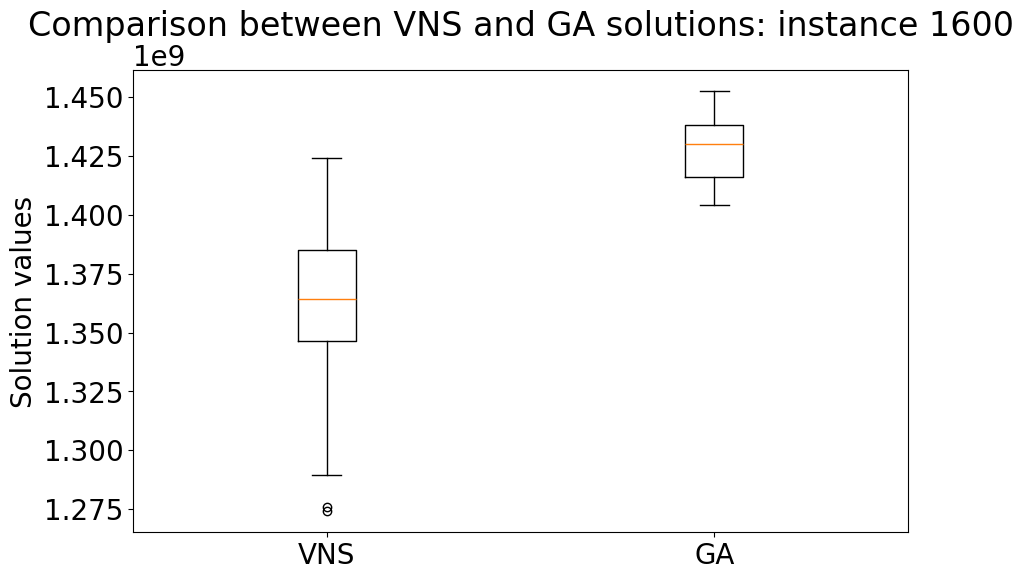
\includegraphics[width=0.45\textwidth]{./imgs/VNSxGA_1600.png} 
      } \\
      \multicolumn{2}{c}{(e) $I, J, K, E, S, Q, N1, N2, N3, M = 1600$} \\
  \end{tabular}
  \caption{ Boxplot visualizations comparing the performance of the VNS algorithm and a population-based metaheuristic (genetic algorithm) across different problem sizes, based on objective function values.}
  \label{fig:VNSxGA_boxplots}
\end{figure*}

% \begin{table}[hb]
%   \begin{center}
%   \caption{Comparison of the VNS algorithm and a population-based metaheuristic (genetic algorithm) in terms of the average objective function value of the best solutions and the average execution time.}
%   \label{tab:comparison_vns_ga}
%   \begin{tabular}{cccc}
%   \hline
%   Instance & VNS & GA & Difference (\%) \\ \hline
%   100  & $7.41 \times 10^7$  & $7.46 \times 10^7$  & 0.71 \\  
%   200  & $1.50 \times 10^8$  & $1.55 \times 10^8$  & 3.37 \\  
%   400  & $3.08 \times 10^8$  & $3.24 \times 10^8$  & 5.31 \\  
%   800  & $6.57 \times 10^8$  & $6.92 \times 10^8$  & 5.26 \\  
%   1600 & $1.36 \times 10^9$  & $1.43 \times 10^9$  & 4.64 \\ \hline
%   \end{tabular}
%   \end{center}
% \end{table}

\begin{table*}[!htb]
  \caption{Comparison of the VNS algorithm and a population-based metaheuristic (Genetic Algorithm) in terms of the average objective function value of the best solutions and the average execution time.}\label{tab:comparison_vns_ga}
  \begin{tabular*}{\textwidth}{@{\extracolsep\fill}lccccc}
  \toprule%
  & \multicolumn{3}{@{}c@{}}{Objective function evaluation (average)} & \multicolumn{2}{@{}c@{}}{Execution time (average)} \\\cmidrule{2-4}\cmidrule{5-6}%
  Instance & VNS & GA & Difference (\%) & VNS & GA \\
  \midrule
  100  & $7.41 \times 10^6$  & $7.46 \times 10^6$  & 0.71 & 241s  & 6,595s \\
  200  & $1.50 \times 10^8$  & $1.55 \times 10^8$  & 3.37 & 714s  & 14,349s \\
  400  & $3.08 \times 10^8$  & $3.24 \times 10^8$  & 5.31 & 2,016s & 33,941s \\
  800  & $6.57 \times 10^8$  & $6.92 \times 10^8$  & 5.26 & 5,538s & 82,687s \\
  1600 & $1.36 \times 10^9$  & $1.43 \times 10^9$  & 4.64 & 17,767s & 217,958s \\
  \bottomrule 
  \end{tabular*}
\end{table*}

%===============================================================================
\section{Conclusion}
\label{sec:conclusion}

This study presents an optimization model for the pistachio supply chain network, addressing the complexities of managing pistachio products 
and by-products across multiple stages. By integrating production, transportation, and facility operations, the model ensures efficient 
resource allocation while meeting capacity and demand constraints. Formulated as a Mixed-Integer Linear Programming (MILP) problem, it is 
solved using a Variable Neighborhood Search (VNS) algorithm, which explores the solution space through Swap, Reversion, Insertion, and 
Slide neighborhood structures.

Comparative analysis highlights VNS’s superiority over Genetic Algorithms (GA) in both solution quality and computational efficiency, 
especially for large-scale instances where exact methods become impractical due to memory and time limitations.

Future research could explore problem-specific neighborhood operators to enhance VNS performance further. Additionally, a hybrid approach 
combining VNS with exact algorithms could improve both accuracy and efficiency, making the methodology more adaptable across industries.

The code and dataset used in this study are available at \url{https://github.com/raissagd/Pistachio_CLSC}.

%===============================================================================
\fi

\bibliography{ifacconf}   

\end{document}
